\documentclass[12pt,a4paper]{article}

\usepackage[T1]{fontenc} 
\usepackage[utf8]{inputenc}

\usepackage[a4paper]{geometry}
\geometry{hscale=0.85,vscale=0.85,centering}
\usepackage{lmodern}
\usepackage{framed}
\usepackage[framed]{ntheorem}
\usepackage{xcolor}
\usepackage{graphicx}
\graphicspath{ {./img/} }
\usepackage{amssymb}
\usepackage{amsmath}
\usepackage{amsfonts}
\usepackage{dsfont}
\usepackage{young}
\usepackage[document]{ragged2e}
\usepackage[vcentermath]{youngtab}
\usepackage{listings}
\usepackage{titlesec}
\usepackage{pgfplots}
\pgfplotsset{compat=1.12}
\usepackage{url}
\usepackage{hyperref}
\hypersetup{					% setup the hyperref-package options
	breaklinks=true,			% 	- allow line break inside links		%
	colorlinks,
	citecolor=black,
	filecolor=black,
	linkcolor=black,
	urlcolor=black
}
\usepackage{tikz}
\usepackage{subfigure}
\usepackage[francais]{babel}



\titleformat{\section}
{\centering \Large \normalfont \scshape}{\thesection}{1em}{}
\titleformat{\subsection}
{\centering \large \scshape}{\thesubsection}{1em}{}
\titleformat{\subsubsection}
{ \normalsize \scshape}{\thesubsubsection}{1em}{}
\numberwithin{equation}{section}

\setcounter{tocdepth}{2}

\newtheorem{theorem}{Théorème}[section]
\newtheorem{coro}{Corollaire}[section]
\newtheorem{lem}{Lemme}[section]

\newcommand{\T}{\mathfrak{T}}
\renewcommand{\Pr}{\mathbb{P}}
\renewcommand{\epsilon}{\varepsilon}
\newcommand{\E}{\mathbb{E}}
\newcommand{\bP}{\mathbf{P}}
\newcommand{\bE}{\mathbf{E}}
\newcommand{\gSym}{\mathfrak{S}_N}
\newcommand{\lN}{\ell_N}
\newcommand{\C}{\mathbb{C}}
\newcommand{\Tr}{\mathrm{Tr}}
\newcommand{\cqfd}{\begin{flushright} $\Box$ \end{flushright}}
\newcommand{\preuve}{$Preuve.$ }


\title{\scshape \huge Forest Cover Type Prediction}
\author{\textbf{Kevin Zagalo} \\  \url{kevin.zagalo@etu.upmc.fr}  \and \textbf{Ismail Benkirane} \\ \url{ismail.benkirane@etu.upmc.fr}}
\date{}

\begin{document}

	\maketitle
	
{\small Projet pour le cours \textit{Apprentissage Statistique} du LIP6, Sorbonne Université} \hfill Janvier 2019
	
	\hrulefill

	{\small \justify Ce projet a pour but de proposer et tester des modèles pour l'étude de la base de données \textit{Covertype} \footnote{\url{https://archive.ics.uci.edu/ml/datasets/Covertype}}, de 581\,012 instances, avec 54 attributs et 7 classes à prédire, sans données manquantes.\\
	Les attributs sont les suivants : \\
	
		\begin{tabular}{l l p{5.2cm}}
			Nom & Unité & Description \\
			\hline
			\verb!Elevation! & mètres & Altitude \\ 
			\verb!Aspect! & degrés & Orientation \\ 
			\verb!Slope! & degrés & Pente \\
			\verb!Horizontal_Distance_To_Hydrology! & mètres & Distance horizontale au point d’eau le plus proche\\
			\verb!Vertical_Distance_To_Hydrology! & mètres & Distance verticale au point d’eau le plus proche \\
			\verb!Horizontal_Distance_To_Roadways! & mètres & Distance horizontale à la route la plus proche \\
			\verb!Hillshade_9a!m & entier entre 0 et 255 & Ombrage à 9h au solstice d’été \\
			\verb!Hillshade_Noon! & entier entre 0 et 255 & Ombrage à 12h au solstice d'été\\
			\verb!Hillshade_3pm! & entier entre 0 et 255 &  Ombrage à 15h au solstice d'été \\
			\verb!Horizontal_Distance_To_Fire_Points! & mètres & Distance horizontale au départ de feu le plus proche\\
			\verb!Wilderness_Area! & 4 colonnes binaires & Wilderness area designation \\
			\verb!Soil_Type! & 40 colonnes binaires & Type de sol\\
			\verb!Cover_Type! & entier entre 1 et 7 & Classe\\
		\end{tabular}\\
	
	\medskip
	Il s'agit donc d'un problème de classification multi-classe avec 7 classes.
	}
	\medskip
	
	\hrulefill

	\tableofcontents
	
	\newpage
	
	\section{Chargement des données}
	
	On choisit d'utiliser la bibliothèque \verb!pandas! pour charger les données, surtout pour l'analyse préliminaire. \verb!pandas! fournit une panoplie de fonctions pour visualiser les données. \verb!groupby!, \verb!boxplot! et \verb!hist! nous seront fort utiles pour choisir les données que nous exploiterons.\\
	
	\medskip
	\medskip
	
	\quad \quad \quad \verb!df_covtype = pd.read_csv('covtype/archives/covtype.data.gz', header=None,!\\
	\quad \quad \quad \quad \quad \quad \quad \quad \quad \quad \quad \quad \quad  \quad \quad \quad \verb!parse_dates=dict_attributs, compression='gzip')! \\
	
	\medskip
	\medskip
	
	Le problème de ce chargement est qu'il stocke les données en type \verb!str!, il nous faut donc convertir le type des données. C'est ce que font les fonctions \verb!convert_to_listofbool!, \verb!convert_to_int! et \verb!convert_to_float!, que nous appliquons de la manière suivante : \\
	\medskip
	\medskip
	
	\quad \verb!for attribut in dict_attributs:! \\
	
	\quad \quad \verb!if attribut is 'Wilderness_Area':!\\
	\quad \quad \quad \verb!wilderness = convert_to_listofbool(df_covtype[attribut])!\\
	\quad \quad \quad \verb!df_covtype[attribut] = [x.index(1)+1 for x in wilderness]!\\
	
	\quad \quad \verb!elif attribut is 'Soil_Type':!\\
	\quad \quad \quad \verb!soil = convert_to_listofbool(df_covtype[attribut])!\\
	\quad \quad \quad \verb!df_covtype[attribut] = [x.index(1)+1 for x in soil]!\\
	
	\quad \quad \verb!elif attribut in ['Cover_Type','Hillshade_9am','Hillshade_Noon','Hillshade_3pm']:!\\
	\quad \quad \quad \verb!df_covtype[attribut] = convert_to_int(df_covtype[attribut])!\\
	
	\quad \quad \verb!else:!\\
	\quad \quad \quad \verb!df_covtype[attribut] = convert_to_float(df_covtype[attribut])!\\

	
	\subsection{Variables et architecture des données}
	
	 	- \verb!df_covtype! : \textit{DataFrame} de toutes les données non traitées triées par attributs. \\
	 	- \verb!df_bycovtype! : \textit{DataFrame.groupby} de toutes les données triées par attributs et regroupée par classes. \\
	 	- \verb!labels! :\textit{np.array} des étiquettes des types de forêts.\\
	 	- \verb!dict_attributs! : \textit{dictionnaire} qui associe les attributs aux bons index. \\
	 	- \verb!qualitative! : \textit{liste} des attributs des données qualitatives.\\
	 	- \verb!wilderness! et \verb!soil! : \textit{listes} gardant en mémoire les vecteurs binaires pour les remplacer par des entiers.\\
	 	
		 	- \verb!Wilderness_Areas! :
		 	\begin{itemize}
		 		\item 1 : Rawah Wilderness Area
		 		\item 2 : Neota Wilderness Area
		 		\item 3 : Comanche Peak Wilderness Area
		 		\item 4 : Cache la Poudre Wilderness Area
		 	\end{itemize}
		 	
		 	- \verb!Soil_Types! :
		 	\begin{itemize}
		 		\item 1 to 40 : based on the USFS Ecological Landtype Units for this study area
		 	\end{itemize}
	 	
	 	- \verb!forest_cover_types! : 
	 	\begin{itemize}
	 		\item 1 : Spruce/Firze
 			\item 2 : Lodgepole Pine
 			\item 3 : Ponderosa Pine
 			\item 4 : Cottonwood/Willow
 			\item 5 : Aspen
 			\item 6 : Douglas-fir
 			\item 7 : Krummholz
		\end{itemize}
	
	
	\subsection{Transformation des données qualitatives}
	On préfèrera garder dans le DataFrame \verb!df_covtype! des entiers plutôt que des vecteurs binaires, quitte à les y remettre dans les données de train et de test ensuite. Cela facilitera grandement l'analyse préliminaire. On utilisera donc \verb!wilderness! et \verb!soil! uniquement pour la partie test des modèles.
	
	\begin{figure}[h]
		\centering
		\includegraphics[width=1\linewidth]{"./img/Dataframe"}
		\caption{Quelques attributs du DataFrame}
		\label{fig:dataframe}
	\end{figure}


	\section{Analyse préliminaire et pré-traitement des données}
	
	Tout d'abord on constate que les données sont inégalement réparties selon les classes. Cela peut vouloir dire plusieurs choses : soit nos données sont mal échantillonnées, soit les types \verb!1! et \verb!2! sont effectivement largement plus répandues. C'est quelque chose dont nous n'avons pas la maitrise, une discussion avec un expert sur le sujet serait préférable. Nous continuerons l'étude sans experts et en supposant que les données sont raisonnablement échantillonnées.
	
	\begin{figure}[h]
		\centering
		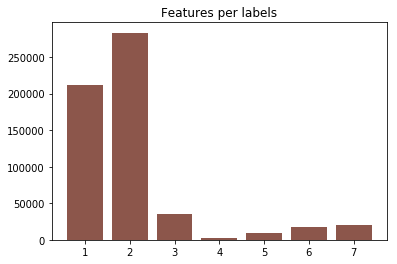
\includegraphics[width=0.7\linewidth]{img/data_hist}
		\caption{Histogramme des données par types de forêts}
		\label{fig:datahist}
	\end{figure}
	
	Au vu du nombres de paramètres que comportent les attributs \verb!Soil_Type! et \verb!Wilderness_Area!, on peut se demander si les garder est vraiment utile.
	
	\begin{figure}
		\centering
		\subfigure[Classe 1]{
			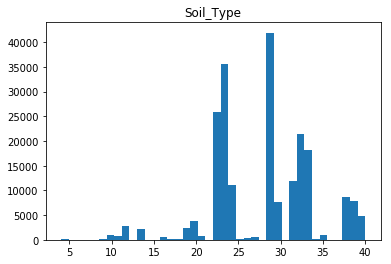
\includegraphics[width=0.3\linewidth]{img/soil1}
			\label{fig:soil1}
		}
	\hfill
		\subfigure[Classe 2]{
			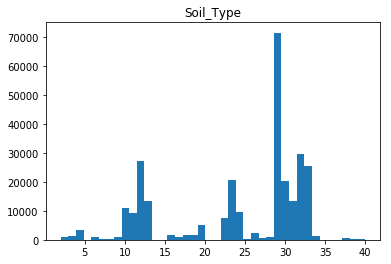
\includegraphics[width=0.3\linewidth]{img/soil2}
			\label{fig:soil2}
		}
	\hfill
		\subfigure[Classe 3]{
			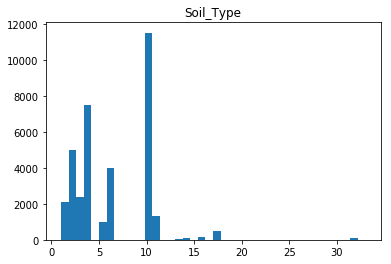
\includegraphics[width=0.3\linewidth]{img/soil3}
			\label{fig:soil3}
		}

	\medskip
	
	\subfigure[Classe 4]{
		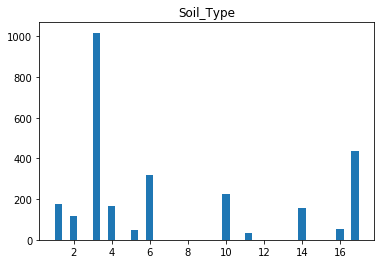
\includegraphics[width=0.22\linewidth]{img/soil4}
		\label{fig:soil4}
	}
	\subfigure[Classe 5]{
		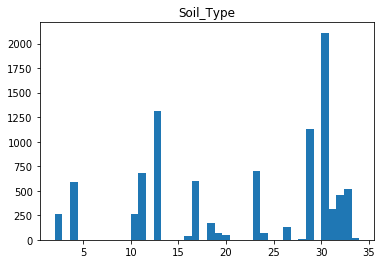
\includegraphics[width=0.22\linewidth]{img/soil5}
		\label{fig:soil5}
	}
	\subfigure[Classe 6]{
		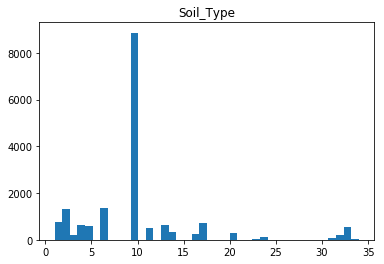
\includegraphics[width=0.22\linewidth]{img/soil6}
		\label{fig:soil6}
	}
	\subfigure[Classe 7]{
		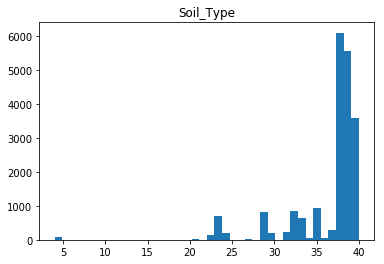
\includegraphics[width=0.22\linewidth]{img/soil7}
		\label{fig:soil7}
	}

	\caption{Distribution des types de sols par classe de forêts}
\end{figure}

	\begin{figure}
	\centering
	\subfigure[Classe 1]{
		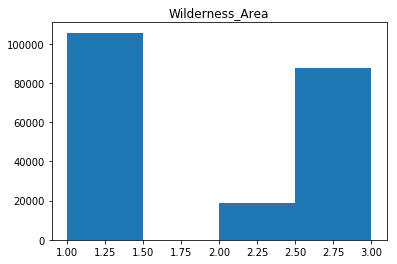
\includegraphics[width=0.3\linewidth]{img/wilderness1}
		\label{fig:wilderness1}
	}
	\hfill
	\subfigure[Classe 2]{
		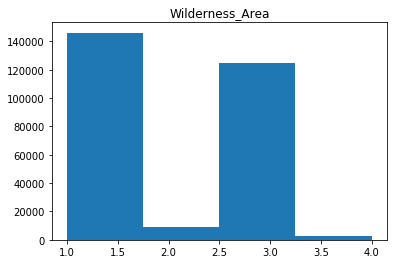
\includegraphics[width=0.3\linewidth]{img/wilderness2}
		\label{fig:wilderness2}
	}
	\hfill
	\subfigure[Classe 3]{
		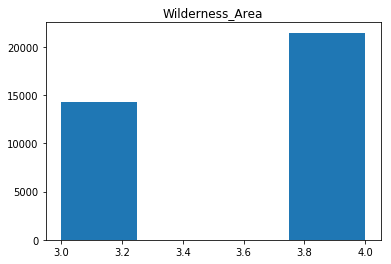
\includegraphics[width=0.3\linewidth]{img/wilderness3}
		\label{fig:wilderness3}
	}
	
	\medskip
	
	\subfigure[Classe 4]{
		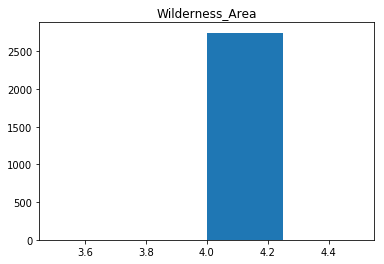
\includegraphics[width=0.22\linewidth]{img/wilderness4}
		\label{fig:wilderness4}
	}
	\subfigure[Classe 5]{
		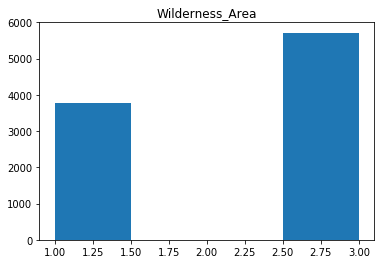
\includegraphics[width=0.22\linewidth]{img/wilderness5}
		\label{fig:wilderness5}
	}
	\subfigure[Classe 6]{
		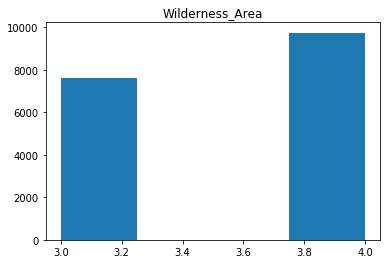
\includegraphics[width=0.22\linewidth]{img/wilderness6}
		\label{fig:wilderness6}
	}
	\subfigure[Classe 7]{
		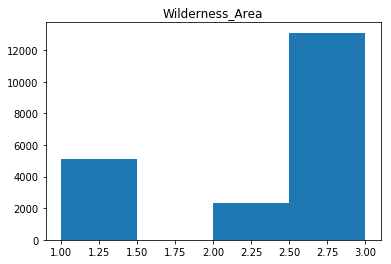
\includegraphics[width=0.22\linewidth]{img/wilderness7}
		\label{fig:wilderness7}
	}
	
	\caption{Distribution de l'attribut Wilderness par classe de forêts}
\end{figure}
		
	\section{Test de différents modèles}
	
	\end{document}